\subsection{a}

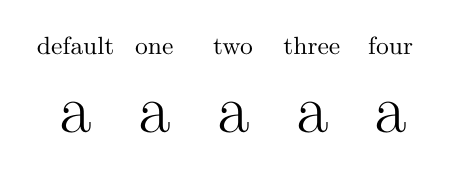
\begin{tikzpicture}
  \def\ssclasses{{"default","one","two","three","four"}}

  \foreach \i in {0,1,...,4} {
    \node[anchor=base] at (\i, 0) {
      \Huge
      % using pgfmathparse to retrieve by index
      \pgfmathparse{\ssclasses[\i]}
      %\pgfmathresult
      \csname ss\pgfmathresult \endcsname a
    };
    \node[anchor=base] at (\i, 1) {
      \small
      \pgfmathparse{\ssclasses[\i]}
      \pgfmathresult
    };
  }
\end{tikzpicture}

The word ``area" presented by default as {\ssdefault area} is hardly
distinguishable from {\ssdefault oreo} (``oreo") which is why a typesetter may
decide to use one of the stylistic alternates for ``a" to produce
{\ssdefault{\ssone a}re{\ssone a}} (ss01),
{\ssdefault{\ssthree a}re{\ssthree a}} (ss03) or
{\ssdefault{\ssfour a}re{\ssfour a}} (ss04).

The ss02 and ss05 alternatives look more like ``dred" or ``drod", respectively
{\ssdefault{\sstwo a}re{\sstwo a}} (ss02) or
{\ssdefault{\ssfive a}re{\ssfive a}} (ss05)
which fails to improve legibility in this particular case.

The following sections discuss the stylistic alternates available for ``a" and
presents some cases where these alternates may prove effective.

\subsubsection{default {\ssdefault a}}

The glyph's double-story design harmonizes well with the overal design
language of the typeface but fails in avoiding ambiguity between letterforms
when this particular glyph is surrounded by letters with a rectangular profile
that happen to be as tall as the x-height as evident in the presentation of the
word \mbox{{\ssdefault area} (area)} which may easily be confused for ``oreo",
``drod'' or ``dred". The arc of the double-story ``a" is not completed due to
the restrictions imposed by the grid that characters are designed unto.

Conversely
\mbox{{\ssdefault train} (train)} or
\mbox{{\ssdefault transport} (transport)}
are rather clearly legible in part due to the distinctive shapes of the words
in question.

\subsubsection{{\ssone a}.ss01}

The ss01 stylistic alternate provides a rectiliniear spur that may at times be
misread as ``o" as in \mbox{\ssdefault m{\ssone aa}g} (maag). The advantage of
this glyph is that it can be used to maintain the horizontal flow of a disinctive
wordforms as evident in
%\mbox{{\ssdefault{\ssone a}rea} (area)},
\mbox{{\ssdefault d{\ssone a}ddy} (daddy)},
\mbox{{\ssdefault {\ssone a}lphabet} (alphabet)},
\mbox{{\ssdefault {\ssone a}lph{\ssone a}bet} (alphabet)},
\mbox{{\ssdefault {\ssone a}llah} (allah)} and
\mbox{{\ssdefault {\ssone a}ll{\ssone a}h} (allah)}.

One point of concern with this rendition of ``a" is that the connection to the
succeeding glyph may need to be ``repaired" through the use of some form of a
ligature as there is not guarantee that separate glyphs will be rendered to
produce a seamless connection.

\subsubsection{{\sstwo a}.ss02}

Another attempt at a double story ``a" provides a more pronounced onset of
the arc but the rectiliniear nature of this feature does not convey the sense
of movement or implied continuation which in many cases inadvertently coaxes
the readers towards a ``d" as in
\mbox{{\ssdefault {\sstwo a}orta} (aorta)},
\mbox{{\ssdefault {\sstwo a}ort{\sstwo a}} (aorta)} or
\mbox{{\sstwo aero} (aero)}
until, for instance, a glyph with a taller ascender such as a ``d" or ``b"
preceeds or succeeds the glyph in question in order to provide the reader with
some visual context as evident in
\mbox{{\sstwo ability} (ability)},
\mbox{{\sstwo data} (data)},
\mbox{{\sstwo dragon} (dragon)}. Note that some readers will face
difficulty reading \mbox{{\sstwo land} (land)} or
\mbox{{\sstwo poland} (poland)} whereas \mbox{{\sstwo deutschland} (deutschland)} or
\mbox{{\sstwo wonderland} (wonderland)}
will be read with minimal effort which may be due to the initial
characters minimizing the search space for word possibilities and therefore
introducing a strong bias that depends less on the interpretation of the
individual letterforms for the interpretation of the word as a whole.

\subsubsection{{\ssthree a}.ss03}
The horizontal spur sloped upwards may at times still be confused for an ``o"
and may potentially disrupt the flow of a formerly typeset text since
the space use by this glyph is different as the right bearing has been modified
to partially account for the amount of negative space above the spur.
Representations such as
\mbox{{\ssdefault {\ssthree a}eon} (aeon)},
\mbox{{\ssdefault {\ssthree a}ero} (aero)},
\mbox{{\ssdefault c{\ssthree a}r} (car)} and
\mbox{{\ssdefault c{\ssthree a}ke} (cake)}
demonstrate some of the legibility challenges with the given glyph choice for
the letter ``a". Yet again, a distinctive wordform may prove instrumental in
reducing ambiguity as evident in
\mbox{{\ssdefault p{\ssthree a}nda} (panda)}.

\subsubsection{{\ssfour a}.ss04}
similar to ss03 with the slope of the extension
inverted leading to a shape that is more reminiscient of ``a"
\mbox{{\ssdefault {\ssfour a}eon} (aeon)},
\mbox{{\ssdefault {\ssfour a}ero} (aero)},
\mbox{{\ssdefault c{\ssfour a}r} (car)} and
\mbox{{\ssdefault c{\ssthree a}ke} (cake)}
